% !TEX program = pdflatex
\RequirePackage[l2tabu, orthodox]{nag}
\documentclass{article}

% FONTS
\usepackage[T1]{fontenc}

% Replace default Latin Modern typewriter with its proportional counterpart
% http://www.tug.dk/FontCatalogue/lmoderntypewriterprop/
\renewcommand*\ttdefault{lmvtt}


%%% OPTION 1 - Fourier Math + New Century Schoolbook + ParaType Sans

% % Import Fourier Math (this imposes its own New Century Schoolbook type)
% % http://www.ctan.org/tex-archive/fonts/fouriernc/
%\usepackage{fouriernc}
%\usepackage{amsmath}
% % Replace with TeX Gyre Schola version of New Century Schoolbook (must scale!)
% % http://www.tug.dk/FontCatalogue/tgschola/
%\usepackage[scale=0.92]{tgschola}
%\usepackage[scaled=0.88]{PTSans}

%% OPTION 2 - MathDesign Math + Bitstream Charter + ParaType Sans

% Import MathDesign (this brings along Bitstream Charter)
% http://www.ctan.org/tex-archive/fonts/mathdesign/
\usepackage[bitstream-charter]{mathdesign}
\usepackage{amsmath}
\usepackage[scaled=0.92]{PTSans}


% %%% OPTION 3 - MTPRO 2 Math + Termes Times + ParaType Sans

% \usepackage{tgtermes}
% \usepackage{amsmath}
% \usepackage[subscriptcorrection,
%             amssymbols,
%             mtpbb,
%             mtpcal,
%             nofontinfo  % suppresses all warnings
%            ]{mtpro2}
% \usepackage{scalefnt,letltxmacro}
% \LetLtxMacro{\oldtextsc}{\textsc}
% \renewcommand{\textsc}[1]{\oldtextsc{\scalefont{1.10}#1}}
% \usepackage[scaled=0.92]{PTSans}

% GEOMETRY
\usepackage[
  paper  = letterpaper,
  left   = 1.65in,
  right  = 1.65in,
  top    = 1.0in,
  bottom = 1.0in,
  ]{geometry}

% COLOR
\usepackage[usenames,dvipsnames]{xcolor}
\definecolor{shadecolor}{gray}{0.9}

% SPACING and TEXT
\usepackage[final,expansion=alltext]{microtype}
\usepackage[english]{babel}
\usepackage[parfill]{parskip}
\usepackage{afterpage}
\usepackage{framed}
\usepackage{verbatim}

%redefine the leftbar environment to accept a width and coloring options
\renewenvironment{leftbar}[1][\hsize]
{%
  \def\FrameCommand
  {%
    {\color{Gray}\vrule width 3pt}%
    \hspace{10pt}%
    %\hspace{0pt}\fboxsep=\FrameSep\colorbox{black!10}%
  }%
  \MakeFramed{\hsize#1\advance\hsize-\width\FrameRestore}%
}%
{\endMakeFramed}

% define a paragraph header function
\DeclareRobustCommand{\parhead}[1]{\textbf{#1}~}

% EDITING
% line numbering in left margin
\usepackage{lineno}
\renewcommand\linenumberfont{\normalfont
                             \footnotesize
                             \sffamily
                             \color{SkyBlue}}
% ragged paragraphs in right margin
\usepackage{ragged2e}
\DeclareRobustCommand{\sidenote}[1]{\marginpar{
                                    \RaggedRight
                                    \textcolor{Plum}{\textsf{#1}}}}
% paragraph counter in right margin
\newcommand{\parnum}{\bfseries\P\arabic{parcount}}
\newcounter{parcount}
\newcommand\p{%
    \stepcounter{parcount}%
    \leavevmode\marginpar[\hfill\parnum]{\parnum}%
}
% paragraph helper
%\DeclareRobustCommand{\PP}{\textcolor{Plum}{\P} }

% COUNTERS
\renewcommand{\labelenumi}{\color{black!67}{\arabic{enumi}.}}
\renewcommand{\labelenumii}{{\color{black!67}(\alph{enumii})}}
\renewcommand{\labelitemi}{{\color{black!67}\textbullet}}

% FIGURES
\usepackage{graphicx}
\usepackage[labelfont=bf]{caption}
\usepackage[format=hang]{subcaption}

% TABLES
\usepackage{booktabs}

% ALGORITHMS
\usepackage[algoruled]{algorithm2e}
\usepackage{listings}
\usepackage{fancyvrb}
\fvset{fontsize=\normalsize}

% BIBLIOGRAPHY
\usepackage{natbib}

% HYPERREF
\usepackage[colorlinks,linktoc=all]{hyperref}
\usepackage[all]{hypcap}
\hypersetup{citecolor=MidnightBlue}
\hypersetup{linkcolor=MidnightBlue}
\hypersetup{urlcolor=MidnightBlue}

% CLEVEREF must come after HYPERREF
\usepackage[nameinlink]{cleveref}

% ACRONYMS
\usepackage[acronym,smallcaps,nowarn]{glossaries}
% \makeglossaries

% COLOR DEFINITIONS
\newcommand{\red}[1]{\textcolor{BrickRed}{#1}}
\newcommand{\orange}[1]{\textcolor{BurntOrange}{#1}}
\newcommand{\green}[1]{\textcolor{OliveGreen}{#1}}
\newcommand{\blue}[1]{\textcolor{MidnightBlue}{#1}}
\newcommand{\gray}[1]{\textcolor{black!60}{#1}}

% LISTINGS DEFINTIONS
\lstdefinestyle{mystyle}{
    commentstyle=\color{OliveGreen},
    keywordstyle=\color{BurntOrange},
    numberstyle=\tiny\color{black!60},
    stringstyle=\color{MidnightBlue},
    basicstyle=\ttfamily,
    breakatwhitespace=false,
    breaklines=true,
    captionpos=b,
    keepspaces=true,
    numbers=left,
    numbersep=5pt,
    showspaces=false,
    showstringspaces=false,
    showtabs=false,
    tabsize=2
}
\lstset{style=mystyle}

\usepackage[colorinlistoftodos,
            prependcaption,
            textsize=tiny,
            backgroundcolor=yellow,
            linecolor=lightgray,
            bordercolor=lightgray]{todonotes}
\DeclareRobustCommand{\mb}[1]{\ensuremath{\boldsymbol{\mathbf{#1}}}}
\DeclareRobustCommand{\KL}[2]{\ensuremath{\textrm{KL}\left(#1\;\|\;#2\right)}}

\newcommand{\supp}{\textrm{supp}}

\newcommand{\E}{\mathbb{E}}
\newcommand{\Var}{\mathbb{V}\textrm{ar}}

% Redundant with reals, naturals, below
\newcommand{\bbN}{\mathbb{N}}
\newcommand{\bbZ}{\mathbb{Z}}
\newcommand{\bbR}{\mathbb{R}}
\newcommand{\bbS}{\mathbb{S}}


\newcommand{\bA}{\boldsymbol{A}}
\newcommand{\bB}{\boldsymbol{B}}
\newcommand{\bC}{\boldsymbol{C}}
\newcommand{\bD}{\boldsymbol{D}}
\newcommand{\bE}{\boldsymbol{E}}
\newcommand{\bF}{\boldsymbol{F}}
\newcommand{\bG}{\boldsymbol{G}}
\newcommand{\bH}{\boldsymbol{H}}
\newcommand{\bI}{\boldsymbol{I}}
\newcommand{\bJ}{\boldsymbol{J}}
\newcommand{\bK}{\boldsymbol{K}}
\newcommand{\bL}{\boldsymbol{L}}
\newcommand{\bM}{\boldsymbol{M}}
\newcommand{\bN}{\boldsymbol{N}}
\newcommand{\bO}{\boldsymbol{O}}
\newcommand{\bP}{\boldsymbol{P}}
\newcommand{\bQ}{\boldsymbol{Q}}
\newcommand{\bR}{\boldsymbol{R}}
\newcommand{\bS}{\boldsymbol{S}}
\newcommand{\bT}{\boldsymbol{T}}
\newcommand{\bU}{\boldsymbol{U}}
\newcommand{\bV}{\boldsymbol{V}}
\newcommand{\bW}{\boldsymbol{W}}
\newcommand{\bX}{\boldsymbol{X}}
\newcommand{\bY}{\boldsymbol{Y}}
\newcommand{\bZ}{\boldsymbol{Z}}
\newcommand{\ba}{\boldsymbol{a}}
\newcommand{\bb}{\boldsymbol{b}}
\newcommand{\bc}{\boldsymbol{c}}
\newcommand{\bd}{\boldsymbol{d}}
\newcommand{\be}{\boldsymbol{e}}
\newcommand{\bbf}{\boldsymbol{f}}
\newcommand{\bg}{\boldsymbol{g}}
\newcommand{\bh}{\boldsymbol{h}}
\newcommand{\bi}{\boldsymbol{i}}
\newcommand{\bj}{\boldsymbol{j}}
\newcommand{\bk}{\boldsymbol{k}}
\newcommand{\bl}{\boldsymbol{l}}
\newcommand{\bbm}{\boldsymbol{m}}
\newcommand{\bn}{\boldsymbol{n}}
\newcommand{\bo}{\boldsymbol{o}}
\newcommand{\bp}{\boldsymbol{p}}
\newcommand{\bq}{\boldsymbol{q}}
\newcommand{\br}{\boldsymbol{r}}
\newcommand{\bs}{\boldsymbol{s}}
\newcommand{\bt}{\boldsymbol{t}}
\newcommand{\bu}{\boldsymbol{u}}
\newcommand{\bv}{\boldsymbol{v}}
\newcommand{\bw}{\boldsymbol{w}}
\newcommand{\bx}{\boldsymbol{x}}
\newcommand{\by}{\boldsymbol{y}}
\newcommand{\bz}{\boldsymbol{z}}

\newcommand{\balpha}{\boldsymbol{\alpha}}
\newcommand{\bbeta}{\boldsymbol{\beta}}
\newcommand{\boldeta}{\boldsymbol{\eta}}
\newcommand{\bkappa}{\boldsymbol{\kappa}}
\newcommand{\bgamma}{\boldsymbol{\gamma}}
\newcommand{\blambda}{\boldsymbol{\lambda}}
\newcommand{\bmu}{\boldsymbol{\mu}}
\newcommand{\bnu}{\boldsymbol{\nu}}
\newcommand{\brho}{\boldsymbol{\rho}}
\newcommand{\bphi}{\boldsymbol{\phi}}
\newcommand{\bpi}{\boldsymbol{\pi}}
\newcommand{\bpsi}{\boldsymbol{\psi}}
\newcommand{\bsigma}{\boldsymbol{\sigma}}
\newcommand{\btheta}{\boldsymbol{\theta}}
\newcommand{\bomega}{\boldsymbol{\omega}}
\newcommand{\bxi}{\boldsymbol{\xi}}
\newcommand{\bGamma}{\boldsymbol{\Gamma}}
\newcommand{\bLambda}{\boldsymbol{\Lambda}}
\newcommand{\bOmega}{\boldsymbol{\Omega}}
\newcommand{\bPhi}{\boldsymbol{\Phi}}
\newcommand{\bPi}{\boldsymbol{\Pi}}
\newcommand{\bPsi}{\boldsymbol{\Psi}}
\newcommand{\bSigma}{\boldsymbol{\Sigma}}
\newcommand{\bTheta}{\boldsymbol{\Theta}}
\newcommand{\bUpsilon}{\boldsymbol{\Upsilon}}
\newcommand{\bXi}{\boldsymbol{\Xi}}
\newcommand{\bepsilon}{\boldsymbol{\epsilon}}

\newcommand{\mcA}{\mathcal{A}}
\newcommand{\mcB}{\mathcal{B}}
\newcommand{\mcC}{\mathcal{C}}
\newcommand{\mcD}{\mathcal{D}}
\newcommand{\mcE}{\mathcal{E}}
\newcommand{\mcF}{\mathcal{F}}
\newcommand{\mcG}{\mathcal{G}}
\newcommand{\mcH}{\mathcal{H}}
\newcommand{\mcI}{\mathcal{I}}
\newcommand{\mcJ}{\mathcal{J}}
\newcommand{\mcK}{\mathcal{K}}
\newcommand{\mcL}{\mathcal{L}}
\newcommand{\mcM}{\mathcal{M}}
\newcommand{\mcN}{\mathcal{N}}
\newcommand{\mcO}{\mathcal{O}}
\newcommand{\mcP}{\mathcal{P}}
\newcommand{\mcQ}{\mathcal{Q}}
\newcommand{\mcR}{\mathcal{R}}
\newcommand{\mcS}{\mathcal{S}}
\newcommand{\mcT}{\mathcal{T}}
\newcommand{\mcU}{\mathcal{U}}
\newcommand{\mcV}{\mathcal{V}}
\newcommand{\mcW}{\mathcal{W}}
\newcommand{\mcX}{\mathcal{X}}
\newcommand{\mcY}{\mathcal{Y}}
\newcommand{\mcZ}{\mathcal{Z}}

\newcommand{\trans}{\mathsf{T}}
\newcommand{\naturals}{\mathbb{N}}
\newcommand{\reals}{\mathbb{R}}
\def\argmax{\operatornamewithlimits{arg\,max}}
\def\argmin{\operatornamewithlimits{arg\,min}}

\newcommand{\distNormal}{\mathcal{N}}
\newcommand{\distGamma}{\mathrm{Gamma}}
\newcommand{\distBernoulli}{\mathrm{Bern}}
\newcommand{\distBinomial}{\mathrm{Bin}}
\newcommand{\distCategorical}{\mathrm{Cat}}
\newcommand{\distDirichlet}{\mathrm{Dir}}
\newcommand{\distMultinomial}{\mathrm{Mult}}
\newcommand{\distPolyaGamma}{\mathrm{PG}}
\newcommand{\distMNIW}{\mathrm{MNIW}}
\newcommand{\distBeta}{\mathrm{Beta}}

\newcommand{\prt}[1]{\frac{\partial}{\partial #1}}
\newcommand{\deriv}[1]{\frac{\mathrm{d}}{\mathrm{d} #1}}


\newcommand{\TODO}[1]{\textcolor{red}{[TODO: #1]}}

\newcommand{\bbI}{\mathbb{I}}
\newcommand{\bbE}{\mathbb{E}}
\newcommand{\bone}{\boldsymbol{1}}
\newcommand{\bigO}{\mathcal{O}}
\newcommand{\iid}[1]{\stackrel{\text{iid}}{#1}}
\newcommand\indep{\protect\mathpalette{\protect\independenT}{\perp}}
\def\independenT#1#2{\mathrel{\rlap{$#1#2$}\mkern4mu{#1#2}}}
\DeclareMathOperator{\Skew}{Skew}
\DeclareMathOperator{\Symm}{Sym}
\DeclareMathOperator{\tr}{tr}

%\DeclareMathOperator{\KL}{KL}
\newcommand{\given}{\, | \,}

\DeclareMathOperator{\diag}{diag}
\let\vec\relax% Set equal to \relax so that LaTeX thinks it's not defined
\DeclareMathOperator{\vec}{vec}
\let\Re\relax
\DeclareMathOperator{\Re}{\textup{Re}}
\let\Im\relax
\DeclareMathOperator{\Im}{\textup{Im}}

% Backcompat: dif and diff both work
\newcommand*\dif{\mathop{}\!\mathrm{d}}
\newcommand*\diff{\mathop{}\!\mathrm{d}}



% \linenumbers

\title{A Discussion of ``Nonparametric Bayes Modeling of Populations of Networks''\\
by Durante, Dunson, and Vogelstein}
\author{Scott W. Linderman and David M. Blei}
\date{\today}

\begin{document}
\maketitle

\begin{abstract}

\end{abstract}

\section{Introduction}

We congratulate the authors...

\citet{durante2016nonparametric} propose a probabilistic model for
populations of networks.  Let~$\{\bA_n\}_{n=1}^N$ denote a collection
of binary adjacency matrices, with
each~${A_n \in \{0,1\}^{V \times V}}$ representing the observed
connectivity in the~$n$-th network.  ${A_{n,[u,v]}=1}$ indicates that
an edge is observed from vertex~$u$ to vertex~$v$ in
network~$n$.
The~$V$ vertices are shared by all~$N$ networks.\todo{obvious?}
By assumption, these networks are undirected~(${A_{n,[u,v]} \equiv A_{n,[v,u]}}$)
and without self-loops~(${A_{n,[v,v]} \equiv 0}$). Thus, it suffices to model only
the lower triangular entries.

The authors build upon the latent space model (LSM), a canonical model
in probabilistic network analysis \citep{hoff2002latent,
  hoff2008modeling}. An LSM is defined by the following parameters and
latent variables: a bias~${z_{u,v} \in \reals}$ for each edge; an
embedding~${x_v \in \reals^D}$ for each vertex; and a
positive-definite ``scaling''
matrix~${\bLambda = \diag(\blambda)}$,~$\blambda \in \reals_+^D$, that
determines the relative importance of the~$D$ latent dimensions.  For
convenience, let~${\bZ = \{\{z_{u,v}\}_{u=1}^V\}_{v=1}^{u-1}}$ denote
the set of per-connection biases.  Given these parameters and latent
variables, the edges are rendered conditionally independent, each
modeled as a Bernoulli random variable with probability,
\begin{align}
  p(A_{n,[u,v]}=1 \given z_{u,v}, \bx_u, \bx_v, \bLambda)
  &= \sigma(z_{u,v} + \bx_u^\trans \bLambda \bx_v),
  & (u &> v),
\end{align}
where~${\sigma(x) = (1+e^{-x})^{-1}}$ is the logistic function.
Clearly, the per-connection bias terms are only warranted
~when~${N > 1}$; otherwise, the model is over-parameterized.

While LSM's are capable of modeling a variety of individual network
structures---simple Erd\H{o}s-R\'{e}nyi
networks~\citep{erdos1959random}, small-world
networks~\citep{watts1998collective}, scale-free
networks~\citep{barabasi1999emergence}, stochastic block
models~\citep{nowicki2001estimation, airoldi2008mixed}, and more---a
population of networks may exhibit a diversity of such connectivity
patterns.  Mixtures of latent space models, as suggested
by~\citet{durante2016nonparametric}, are naturally suited to this type
of heterogeneous data.

Now let there
be~$H$ separate mixture components, each with 
a unique set of vertex embeddings~${\bx_v^{(h)} \in \reals^D}$
and its own scaling matrix~$\bLambda^{(h)}$. Furthermore,
let~${h_n \in \{1, \ldots, H\}}$ denote the mixture component
to which the~$n$-th network is attributed. 
The likelihood of a network is then
given by,
\begin{align}
  \label{eq:molsm_lkhd}
  p \left(\bA_n \given
    \bZ, \{\{\bx_v^{(h)}\}_{v=1}^V,
  \bLambda^{(h)}\}_{h=1}^H, h_n \right) 
  = \prod_{u=1}^V \prod_{v=1}^{u-1}
  \distBernoulli \left(A_{n,[u,v]} \given
    \sigma(z_{u,v} + \bx_{u}^{(h_n)^\trans} \bLambda^{(h_n)} \bx_v^{(h_n)}) \right),
\end{align}
where~${\distBernoulli(x \given p) = p^x (1-p)^{1-x}}$ is the Bernoulli likelihood function.

% \citet{durante2016nonparametric} provide conditions under which a prior
% distribution on latent variables and parameters will ensure support for
% the entire space of adjacency matrices, which ensures posterior consistency
% as the number of networks~$N$ goes to infinity. Moreover, they use
\citet{durante2016nonparametric} use
P\'{o}lya-gamma augmentation to develop an
efficient Gibbs sampling algorithm for posterior inference in the case
where~$\bx_v^{(h)}$ and~$z_{u,v}$ have Gaussian prior distributions. 
While the Bernoulli likelihoods are not conjugate with these Gaussian
priors, conditioning on the P\'{o}lya-gamma auxiliary variables renders them so.
These auxiliary variables have straightforward and na\"{i}vely parallelizable
updates as well, making the overall algorithm highly efficient.
\todo[inline]{How important is it to list their other contributions? E.g.
  the multiplicative inverse gamma prior to promote sparsity in number of components,
  the theoretical analysis of the support of the prior...}

\section{A Factorial Generalization}
We offer an alternative perspective on the mixture of latent
space models described above.  From this viewpoint, a number
of natural generalizations become clear. Consider the space
formed by combining the embeddings and scalings of the~$H$
mixture components.  Specifically, let
\begin{align}
  \widetilde{\bx}_v &= \left[\bx_v^{(1)^\trans}, \ldots, \bx_v^{(H)^\trans}\right]^\trans, \\
  \widetilde{\blambda} &= \left[\blambda^{(1)^\trans}, \ldots, \blambda^{(H)^\trans} \right]^\trans
\end{align}
denote column vectors in~$\reals^{D \cdot H}$ formed by concatenating the
embeddings and scaling factors of each mixture component, respectively.
Then, introduce a ``mask'' vector for each network defined by,
\begin{align}
  \widetilde{\bbm}_n &= \left[ \bbI[h_n=1] \cdot \bone_D^\trans, \ldots, \bbI[h_n=H] \cdot \bone_D^\trans \right]^\trans,
\end{align}
where~$\bbI[\cdot]$ is an indicator that evaluates to one if its
argument is true and zero otherwise, and~$\bone_D$ is a column vector
of length~$D$ filled with ones. The mask vector represents
the mixture component~$h_n$ as a
vector with exactly~$D$ ones in the coordinates corresponding
to~$\bx_v^{(h_n)}$ and~$\blambda^{(h_n)}$. The likelihood in Eq.~\eqref{eq:molsm_lkhd} can now
be equivalently expressed as,
\begin{align}
  p \left(\bA_n \given
  \bZ, \{\widetilde{\bx}_v\}_{v=1}^V,
  \widetilde{\blambda}, h_n \right) 
  &= \prod_{u=1}^V \prod_{v=1}^{u-1}
  \distBernoulli \left(A_{n,[u,v]} \given
    \sigma \left(z_{u,v} + \widetilde{\bx}_{u}^\trans
    \diag(\widetilde{\blambda} \odot \widetilde{\bbm}_n) \,
    \widetilde{\bx}_v \right) \right),
\end{align}
where~$\odot$ denotes elementwise multiplication. The mask effectively
turns on or off certain dimensions of the latent space according to
the network's mixture assignment~$h_n$.

This suggests an obvious extension: rather than restricting the model
to exactly~$H$ unique masks, instead allow each network to take on any
of thee~$2^{D \cdot H}$ possible binary masks. More generally, let~$K$
denote the total number of latent factors (so far~${K=D \cdot
  H}$). Intuitively, the set of networks is characeterized by~$K$
latent factors; in any given network, only a subset of those factors
play a role in deterimining the edge probabilities. Unlike the mixture
model, in which only~$H$ different subsets of factors are allowed, here any
possible combination of factors can be chosen, making this a strict
generalization of the mixture model.  Moreover, with more flexibility
in the choice of subset, it is likely that~${K < D \cdot H}$
dimensions will suffice for this \emph{factorial latent space model}.

In the finite~$K$ case, a natural prior is
\begin{align}
  \label{eq:prior_m}
  p(\widetilde{\bbm}_n \given \{\rho_k\}_{k=1}^K)
  &=\prod_{k=1}^K \distBernoulli(\widetilde{m}_{n,k} \given \rho_k), \\
  \label{eq:prior_rho}
  p(\rho_k; \alpha) &= \distBeta(\rho_k \given \tfrac{\alpha}{K}, 1), 
\end{align}
where~$\alpha$ is a hyperparameter that controls the sparsity of the
mask matrices.  One of the primary contributions of
\citet{durante2016nonparametric} is a Bayesian nonparametric model
that grows in complexity (number of mixture components, number of
latent dimensions per component) as the data demands.
We achieve similar flexibility here: as~$K$ goes to infinity, the 
prior~\eqref{eq:prior_m}--\eqref{eq:prior_rho} converges to a Bayesian
nonparametric prior known as the Indian buffet process~\citep{griffiths2005infinite}.
Intuitively, each new network has nonzero probability of introducing a
new latent factor, i.e. of increasing the dimensionality of the
embeddings.

Posterior inference in the factorial model requires slight
modifications to the mixture model inference algorithm. Rather than
sampling a mixture identity~$h_n$ for each network, we now must sample
the binary mask~$\widetilde{\bbm}_n$. Assuming a large but finite
value of~$K$---which is akin to the ``weak limit'' approximation used
by~\citet{durante2016nonparametric}---we may Gibbs sample each
coordinate of the mask vector~$\widetilde{m}_{n,k}$ holding the
remainder~$\widetilde{\bbm}_{n,\neg k}$ fixed.  These conditionals are
of the same form as the class conditional probabilities in the mixture
model:
\begin{multline}
  p(\widetilde{m}_{n,k} \given \widetilde{\bbm}_{n, \neg k}, \bA_n, \bZ,
  \{\widetilde{\bx}_v\}_{v=1}^V, \widetilde{\blambda},\rho_k) 
  \propto \distBernoulli(\widetilde{m}_{n,k} \given \rho_k) \times
  p\left(\bA_n \given
  \bZ, \{\widetilde{\bx}_v\}_{v=1}^V,
  \widetilde{\blambda}, \widetilde{\bbm}_n \right) 
\end{multline}
In sampling the binary masks, we effectively sample the number of
factors active in a network.  Thus, sparsity inducing priors
on~$\widetilde{\lambda}_k$ are no longer necessary as they are
superseded by the binary masks.

Of course, we also pay a computational cost in generalizing from
mixtures to factorial models.  In the mixture model, the conditional
distribution of~$h_n$ could be computed exactly, but the conditional
distribution of~$\widetilde{\bbm}_n$ in the factorial model may take
on~$2^K$ values, which will generally be intractable.  One concern is
that the coordinate-wise Gibbs sampler proposed above will suffer poor
mixing. For example,~$\widetilde{m}_{n,k}$ may be highly correlated
with~$\{\widetilde{x}_{v,k}\}_{v=1}^V$, making it hard to turn off
or on a factor while holding the embeddings fixed.\footnote{Note that
  this is also a concern in mixture models where mixture assignments
  may be strongly coupled to the mixture parameters.} In some models
it is possible to address this concern by integrating out the
embeddings when sampling the binary masks; such a collapsed sampler
would also benefit the mixture model.  Unfortunately, due to the
quadratic form in the edge probabilities, this marginalizaiton
does not appear to be straightforward, even after P\'{o}lya-gamma
augmentation.

\section{Experiments}

\begin{figure}[t]
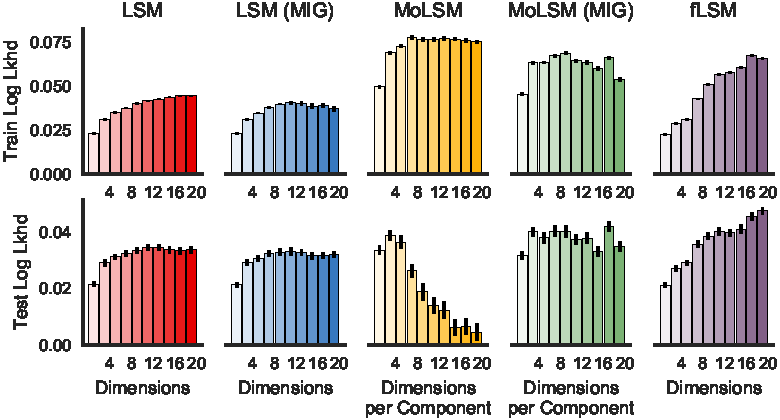
\includegraphics[width=\linewidth]{figures/lls.pdf}
\caption{\textit{Train and test likelihood for various
  latent space models on brain network data.}}
\label{fig:lls}
\end{figure}

\begin{figure}[t]
  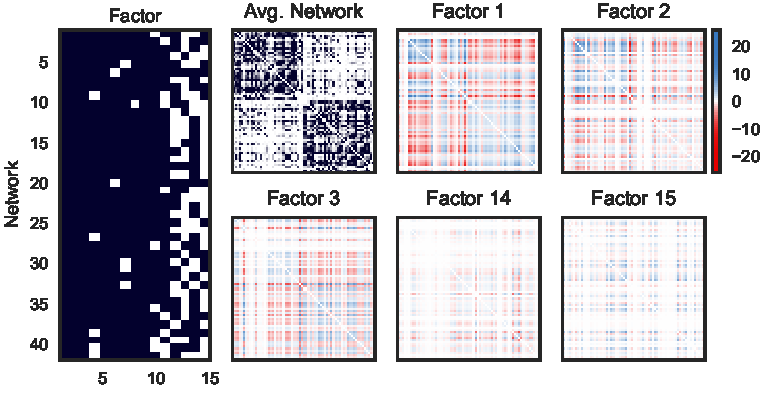
\includegraphics[width=\linewidth]{figures/factors.pdf}
  \vspace{-.4in}
\caption{\textit{Inferred factors of the LSM and their
  usage.}}
\label{fig:lls}
\end{figure}

\section{Conclusion}
\citet{durante2016nonparametric} present a mixture of latent space
models for capturing low-dimensional structure in populations of
networks.  Mixing over latent embeddings naturally handles network-to-network
variability within the population and provides promising results
compared to other hierarchical models that assume a single set of
edge probabilities across all networks.  Moreover, their Bayesian
nonparametric approach allows flexible inference of the number of
mixture components and latent dimensions in a data-driven manner.
We commend them on their work.

We present a straightforward generalization from their mixture
model to a \emph{factorial} model in which the population of
networks share a set of latent factors, but only a subset of those
factors actively determine edge probabilities for any given network.
For example, in studying brain connectivity, the factorial model postulates
that a set of latent features determines the probability of fiber
tracts between two brain regions (e.g. age, diseases, drug use), and
each patient may possess a different subset of these features. By contrast,
the mixture model postulates a collection of different ``types'' of
patients, each with characteristic patterns of connectivity.  Clearly
these two models are quite similar, but they may yield different
insights into the population of networks under study.





\bibliographystyle{apa}
\bibliography{refs.bib}

\end{document}






































